\documentclass[11pt,a4paper]{article}
\usepackage[margin=1.7cm]{geometry}
\usepackage{amsmath,amssymb,mathtools}
\usepackage{xcolor}
\usepackage{tcolorbox}
\usepackage{enumitem}
\usepackage{tikz}
\usetikzlibrary{positioning}
\usepackage{fancyhdr}
\usepackage{titlesec}
\usepackage{array}
\usepackage{booktabs}
\usepackage[hidelinks]{hyperref}
\usepackage{lmodern}
\setlength{\parindent}{0pt}
\setlength{\parskip}{5pt}
\definecolor{navy}{HTML}{17365D}
\definecolor{blue}{HTML}{DCEBFA}
\definecolor{green}{HTML}{E5F4E3}
\definecolor{gold}{HTML}{FFF2CC}
\definecolor{redbox}{HTML}{FCE8E6}
\definecolor{grey}{HTML}{F4F5F7}

\pagestyle{fancy}
\fancyhf{}
\lhead{\textbf{MATH6342 Linear Systems}}
\rhead{Week 1 Guide}
\cfoot{\thepage}
\renewcommand{\headrulewidth}{0.4pt}

\titleformat{\section}{\Large\bfseries\color{navy}}{}{0pt}{}
\titleformat{\subsection}{\large\bfseries\color{navy}}{}{0pt}{}

\newtcolorbox{keybox}[1][]{colback=blue,colframe=navy,boxrule=0.8pt,arc=2mm,title=\textbf{#1}}
\newtcolorbox{rememberbox}[1][]{colback=green,colframe=green!45!black,boxrule=0.8pt,arc=2mm,title=\textbf{#1}}
\newtcolorbox{exam}[1][]{colback=gold,colframe=orange!70!black,boxrule=0.8pt,arc=2mm,title=\textbf{#1}}
\newtcolorbox{note}[1][]{colback=grey,colframe=gray!60,boxrule=0.6pt,arc=2mm,title=\textbf{#1}}

\begin{document}

\begin{center}
{\Huge\bfseries\color{navy} MATH6342 Linear Systems}\\[4pt]
{\LARGE Week 1: What You Are Likely to Cover}\\[8pt]
{\large Simplified preparation and revision guide}
\end{center}

\begin{note}[Important]
The uploaded MATH6342 files are organised by \emph{frames/chapters}, not by teaching week. Therefore this guide treats the opening part of Chapter 1 (``Linear systems and their description'', frames 6--30) as the likely Week 1 material. The exact stopping point may differ slightly depending on lecture pace.
\end{note}

\section{1. The big idea of Week 1}

The course starts by thinking of a system as a ``machine'' that evolves in time. The system receives an \textbf{input}, has an internal \textbf{state}, and produces an \textbf{output}.

\begin{center}
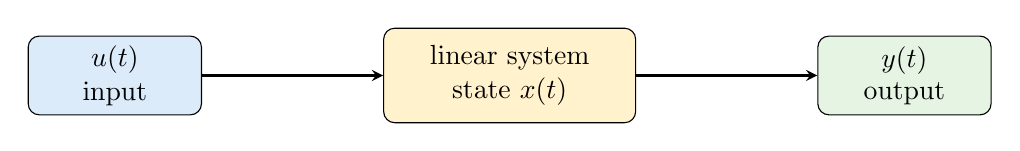
\begin{tikzpicture}[>=stealth, node distance=2.3cm]
\node[draw,rounded corners,fill=blue,minimum width=2.2cm,minimum height=1cm] (u) {\shortstack{$u(t)$\\ input}};
\node[draw,rounded corners,fill=gold,right=of u,minimum width=3.2cm,minimum height=1.2cm] (sys) {\shortstack{linear system\\ state $x(t)$}};
\node[draw,rounded corners,fill=green,right=of sys,minimum width=2.2cm,minimum height=1cm] (y) {\shortstack{$y(t)$\\ output}};
\draw[->,thick] (u) -- (sys);
\draw[->,thick] (sys) -- (y);
\end{tikzpicture}
\end{center}

The central question is:
\[
\boxed{\text{How does the input }u(t)\text{ determine the output }y(t)?}
\]

Examples mentioned in the notes include wind turbines, heating systems, electrical networks, vehicle suspension, epidemics, predator--prey systems and musical filters.

\begin{keybox}[Core language]
\textbf{Input $u(t)$:} the signal or forcing applied to the system.\\
\textbf{State $x(t)$:} variables that describe the internal condition of the system.\\
\textbf{Output $y(t)$:} what the system produces or what we observe.
\end{keybox}

\section{2. Linear operators}

A map $L:V\to W$ is linear if
\[
L(\lambda f+\mu g)=\lambda Lf+\mu Lg.
\]

You will see familiar calculus operations viewed as \emph{linear operators}:

\begin{center}
\begin{tabular}{>{\bfseries}p{4cm} p{7.5cm}}
\toprule
Operation & What it does \\
\midrule
Differentiation & $f\mapsto \dfrac{df}{dt}$ \\
Integration & $f\mapsto \displaystyle\int_0^x f(t)\,dt$ \\
Amplification & $f\mapsto af$, for constant $a$ \\
Multiplication & $f\mapsto h(t)f(t)$ \\
Evaluation & $f\mapsto f(t_0)$ \\
\bottomrule
\end{tabular}
\end{center}

\begin{rememberbox}[Why this matters]
Block diagrams are built by connecting simple linear operations. Instead of seeing a long differential equation as one intimidating object, you break it into small pieces: multiply, add, differentiate and integrate.
\end{rememberbox}

\section{3. Block diagrams}

A major new skill is learning to \textbf{read and draw block diagrams}.

The basic building blocks are:
\begin{itemize}[leftmargin=1.2cm]
\item \textbf{Amplifier:} $u\mapsto au$.
\item \textbf{Integrator:} $u\mapsto \int u$.
\item \textbf{Differentiator:} $u\mapsto \dfrac{du}{dt}$.
\item \textbf{Summing junction:} combines signals, e.g. $u_1+u_2$.
\item \textbf{Tap:} copies a signal into another branch without dividing its value.
\end{itemize}

For example, the notes represent
\[
y=3\int u+2u'+6u
\]
by splitting the input into several branches, applying the required operation to each branch, and adding the results.

\begin{exam}[Week 1 skill to practise]
Given an equation, try to identify the separate operations needed to construct its block diagram. Conversely, when shown a block diagram, follow each branch and reconstruct the equation for the output.
\end{exam}

\newpage
\section{4. Open-loop and feedback systems}

\subsection{Open-loop}
An open-loop system processes the input and produces an output, but the output is \textbf{not fed back} into the system.

Conceptually:
\[
u \longrightarrow \boxed{\text{system}} \longrightarrow y.
\]

\subsection{Closed-loop / feedback}
In a feedback system, part of the output is returned to the input side and influences future behaviour.

\begin{center}
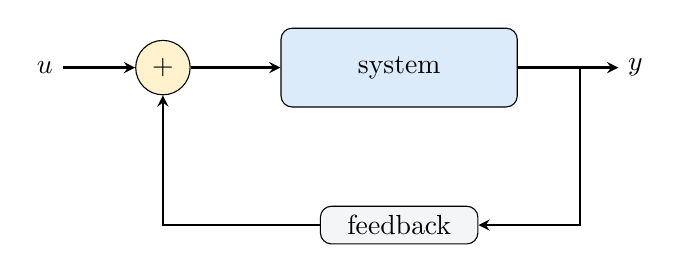
\begin{tikzpicture}[>=stealth]
\node[draw,circle,fill=gold] (sum) at (0,0) {$+$};
\node[draw,rounded corners,fill=blue,minimum width=3cm,minimum height=1cm] (sys) at (3,0) {system};
\node (out) at (6,0) {$y$};
\node[draw,rounded corners,fill=grey,minimum width=2cm] (fb) at (3,-2) {feedback};
\node (in) at (-1.5,0) {$u$};
\draw[->,thick] (in) -- (sum);
\draw[->,thick] (sum) -- (sys);
\draw[->,thick] (sys) -- (out);
\draw[->,thick] (5.3,0) |- (fb);
\draw[->,thick] (fb) -| (sum);
\end{tikzpicture}
\end{center}

\begin{keybox}[Positive feedback]
The returned output reinforces the behaviour of the system. Example from the notes:
\[
\frac{dx}{dt}=kx+u,\qquad k>0.
\]
A larger state $x$ creates further growth.
\end{keybox}

\begin{keybox}[Negative feedback]
The returned signal opposes change and can stabilise behaviour. For the cyclist example,
\[
m\frac{dv}{dt}=-kv+u.
\]
The faster the cyclist moves, the larger the opposing air-resistance term $-kv$.
\end{keybox}

\section{5. Linear differential equations as systems}

The course next connects block diagrams with differential equations. A general linear differential operator has the form
\[
Lf(t)=a_n(t)\frac{d^nf}{dt^n}+a_{n-1}(t)\frac{d^{n-1}f}{dt^{n-1}}+\cdots+a_0(t)f(t).
\]

For constant coefficients, equations of the form
\[
a_ny^{(n)}+\cdots+a_0y
=b_mu^{(m)}+\cdots+b_0u
\]
can be realised using amplifiers, summing junctions, integrators and differentiators.

\begin{rememberbox}[What the lecturer is trying to show]
A differential equation is not just an equation to solve. It can also be interpreted as a \textbf{network of connected linear operations}. This point of view becomes important later for control systems.
\end{rememberbox}

\section{6. The damped harmonic oscillator}

A key example that appears early and returns later is
\[
\boxed{y''+\beta y'+\gamma y=u.}
\]

Interpretation:
\begin{itemize}[leftmargin=1.2cm]
\item $y$ = displacement,
\item $y'$ = velocity,
\item $y''$ = acceleration,
\item $u(t)$ = external driving force,
\item $-\gamma y$ = restoring force from a spring,
\item $-\beta y'$ = damping from a shock absorber.
\end{itemize}

The notes use vehicle suspension as a physical example.

\newpage
\section{7. From a second-order ODE to a matrix system}

This is one of the most important ideas to understand early.

Start with
\[
y''+\beta y'+\gamma y=u.
\]
Introduce a new variable
\[
v=y'.
\]
Then
\[
\begin{aligned}
y'&=v,\\
v'&=-\beta v-\gamma y+u.
\end{aligned}
\]

Now define
\[
X=\begin{pmatrix}y\\v\end{pmatrix},\qquad
A=\begin{pmatrix}0&1\\-\gamma&-\beta\end{pmatrix},\qquad
B=\begin{pmatrix}0\\1\end{pmatrix}.
\]
Then the entire second-order equation becomes
\[
\boxed{\frac{dX}{dt}=AX+Bu.}
\]

\begin{exam}[This is worth learning carefully]
The general idea is called \textbf{reduction of order}: an $n$th-order scalar differential equation can be rewritten as a first-order vector equation
\[
\frac{dX}{dt}=AX+Bu.
\]
This lets the course use linear algebra to study differential equations.
\end{exam}

\section{8. What you should know by the end of Week 1}

You should aim to be able to:
\begin{enumerate}[leftmargin=1.2cm]
\item explain the meaning of input, state and output;
\item recognise examples of linear systems;
\item state what it means for an operator to be linear;
\item recognise amplifiers, integrators, differentiators, taps and summing junctions;
\item translate simple equations into block diagrams and back;
\item distinguish open-loop and closed-loop/feedback systems;
\item explain positive versus negative feedback;
\item understand how a differential equation can be viewed as a feedback system;
\item rewrite a second-order ODE as a first-order matrix system;
\item recognise the state-space form $X'=AX+Bu$.
\end{enumerate}

\section{9. What to revise before the lecture}

\begin{center}
\begin{tabular}{p{5cm}p{7cm}}
\toprule
\textbf{Topic} & \textbf{What you need}\\
\midrule
Linear algebra & matrix multiplication, matrix-vector multiplication, $2\times 2$ matrices \\
Calculus & derivatives and integrals \\
ODEs & notation such as $y',y'',y^{(n)}$ and basic first/second-order ODEs \\
Linear maps & understanding $L(\lambda f+\mu g)=\lambda Lf+\mu Lg$ \\
Complex numbers & only basic familiarity at this stage \\
\bottomrule
\end{tabular}
\end{center}

\begin{rememberbox}[The Week 1 picture in one line]
\[
\boxed{\text{ODEs} \quad\longleftrightarrow\quad \text{block diagrams} \quad\longleftrightarrow\quad \text{matrix systems}}
\]
That connection is the foundation for the rest of MATH6342.
\end{rememberbox}

\section{10. Quick self-test}

Try these without looking back:
\begin{enumerate}[leftmargin=1.2cm]
\item What are the input, state and output of a system?
\item What does an amplifier block labelled $a$ do to a signal $u$?
\item What is the difference between a tap and a summing junction?
\item What makes a system a feedback system?
\item Is $m v'=-kv+u$ an example of positive or negative feedback?
\item Rewrite $y''+3y'+2y=u$ as a system of two first-order equations.
\item Write that system in the form $X'=AX+Bu$.
\end{enumerate}

\begin{note}[Source]
Prepared from the uploaded Lancaster University MATH6342 \emph{Linear systems} lecture notes and beamer slides (2026/27), especially Chapter 1: frames 6--30. The files do not explicitly label a ``Week 1'', so the week boundary in this guide is inferred from the opening sequence of the module.
\end{note}

\end{document}
